\documentclass[10pt]{article}
\usepackage[margin=17mm]{geometry}
\usepackage{graphicx,booktabs,hyperref}
\usepackage[strings]{underscore}
\setlength{\parindent}{0pt}\setlength{\parskip}{5pt}
\begin{document}
\section*{ell=8 draw 6: zero-guess degree-four refutation}
First registered 200k-cap pilot, 2026-10-25; protocol and sequential
runner committed at f83ed00d8 before execution. Original ell=8 UNSAT draw 6,
(m,n,ell)=(3,22,8), frozen input unchanged, no guessed variables. Degree-four
dense closure returns refuted. This is an observed zero-guess refutation
for this input; independent solver/cost replay is still outstanding.

\begin{center}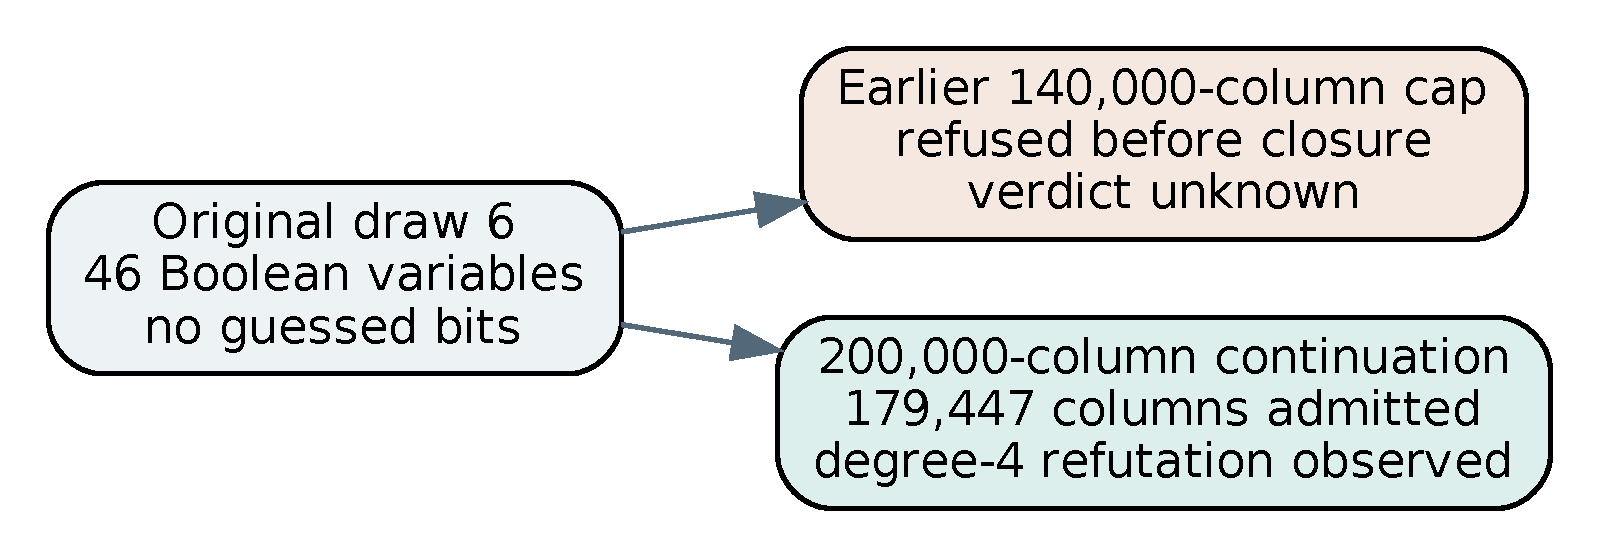
\includegraphics[width=.98\linewidth]{cap-diagram.pdf}\end{center}

Native recorded columns: 179,447; terminal rank 1.
Charged closure products: 616,309; solver-word operations:
1,548,633,051,630. Every branch of this zero-guess cell is charged
(one branch). These are solver-stage counts, not complete decomposition or
DLP costs. A single comparable cell gets a resource-gate diagram instead
of a fitted cost curve. The prior cap refusal is retained, not a failed
refutation or zero-cost comparison. Raising the cap is not an algorithmic gain.

The result shows that the upstream all-branches four-guess observation is
not evidence that four guesses are necessary on every fixture. Draw 0 still
has eight nonrefuting balanced k=3 branches; minima for other inputs and
variable sets remain unresolved. No universal degree law or scaling claim
is made. The 115 remaining registered attempts were ongoing when this pilot
snapshot was made, with individual caps/failures retained.

The independent fixture audit counts zero Boolean solutions and finds this
target abscissa liftable on E0 over GF($2^{22}$). Target/base subgroup
membership remains unknown. A curve lift does not make this a verified
subgroup-decomposition query or a full IC relation.

Resources: unchanged 12-GiB address-space and 900-second limits, four Rayon
threads, shared host L0; diagnostic time is in the raw row and resource receipt.
Frozen instrument SHA-256 starts ab544a41; build source d67f6085, with the later
source-only parity lint change excluded. Full hashes and command are archived.

Raw cell: \path{../../runs/guess-cap200k-20261025-01/cell-0000-d6-k0-b0/}.
Stable pilot snapshot under evidence/: \path{runs-local-followup-20261025-01.tar.xz}.
Original input: \path{../../inputs/guess-ell8.jsonl}.
Protocol: \path{../../GUESS_CAP200K_PROTOCOL.md}.
The original 33-run archive and all earlier reports stay unchanged.

\end{document}
